\begin{table*}[t]
\centering\small
\caption{Frozen new-period results: count-fraction CRPS and ratio-9 reserve loss, both multiplied by 1,000 (lower is better). Each source has 28 origins. All joint arms share its development-selected three-seed marginal predictor. Direct rows use exact count distributions. Last row: typed Student-$t$ (UCI), subscription-only Gaussian (Azure), team-only Gaussian (BPI14), selected on development, never on confirmation.}\label{tab:extension-counts}
\begin{tabular}{lrrrrrr}
\toprule
Model & UCI CRPS & Loss & Azure CRPS & Loss & BPI14 CRPS & Loss \\
\midrule
Independent & 48.63 & 148.60 & 8.70 & 20.83 & 34.76 & 81.82 \\
Gaussian global & 44.57 & 92.39 & 7.60 & 14.20 & 34.15 & 85.89 \\
Gaussian typed & 43.11 & 90.42 & 7.60 & 14.20 & 34.08 & 86.14 \\
Shuffled typed & 46.41 & 117.50 & 7.60 & 14.20 & 34.22 & 86.48 \\
Student-$t$ global & 44.44 & 91.18 & 7.58 & 14.17 & 34.41 & 87.91 \\
Student-$t$ typed & 42.84 & 84.72 & 7.58 & 14.17 & 34.40 & 88.25 \\
Direct DM (exact) & 43.31 & 87.15 & 7.47 & 13.19 & 33.70 & 82.46 \\
Bias-DM (exact) & 42.77 & 86.02 & 7.44 & 13.11 & 36.11 & 85.51 \\
Residual & 46.57 & 122.43 & 9.76 & 32.56 & 39.11 & 94.63 \\
Dev.-selected coherent & 42.84 & 84.72 & 7.25 & 13.00 & 33.74 & 78.76 \\
\bottomrule
\end{tabular}
\end{table*}

\begin{table}[t]
\centering\small
\caption{New-period equal-origin integrated Brier $\times 1,000$ (lower is better), using three-seed mean CDFs. Selected beforehand: typed graph (UCI), temporal HGB (Azure), relational HGB (BPI14). Single-relation order: handler/team for UCI; deployment/subscription for Azure. BPI14 has one relation.}\label{tab:extension-marginals}
\begin{tabular}{lrrr}
\toprule
Marginal model & UCI & Azure & BPI14 \\
\midrule
HGB personal & 69.04 & 6.15 & 72.84 \\
HGB relations & 72.70 & 6.95 & 72.86 \\
HGB temporal & 70.09 & 6.83 & 72.45 \\
Node MLP & 68.07 & 6.40 & 74.14 \\
Global set & 69.24 & 6.59 & 74.83 \\
Typed graph & 67.88 & 6.45 & 74.27 \\
Shuffled graph & 68.67 & 6.60 & --- \\
Relation 1 only & 68.07 & 6.30 & --- \\
Relation 2 only & 67.76 & 6.39 & --- \\
Temporal attention & 66.77 & 6.20 & 72.87 \\
\bottomrule
\end{tabular}
\end{table}

\begin{figure*}[t]
\centering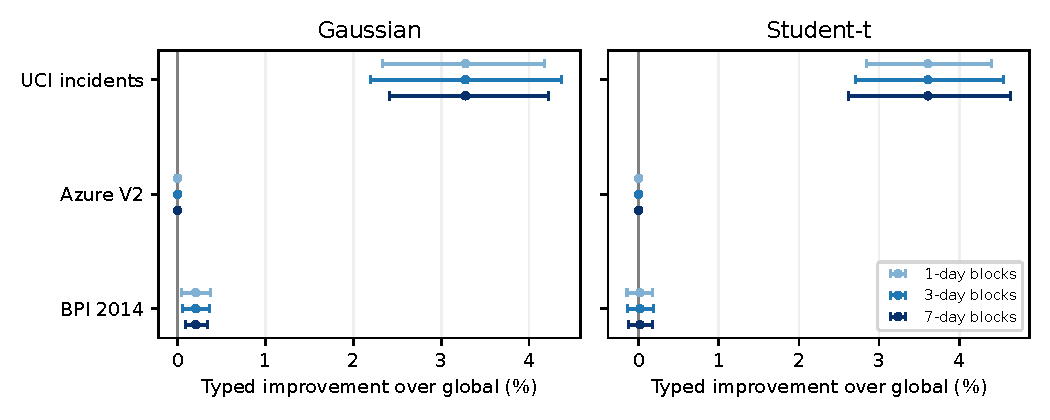
\includegraphics[width=.96\textwidth]{figures/extension_effects.pdf}
\caption{Primary typed-versus-global comparisons in the three new periods.
Positive values favor typed incidence. Bars are descriptive paired 95\%
circular-block intervals, using 1/3/7-day blocks. Azure's combined typed and
global fits are identical; these zero differences do not imply absence of
all relation signal. Its separately fitted subscription-only control is
reported in Table~\ref{tab:extension-relations}. A seven-day Azure block spans
the whole trace, so that sensitivity is degenerate.}
\label{fig:extension}
\end{figure*}

\subsection{Incident relations help, but direct counts remain competitive}
The new frozen periods contain 426,610 repeated entity--origin queries at
84 origins. On UCI incidents, Gaussian typed factors improve count-fraction
CRPS from .04457 to .04311 relative to a global factor, a 3.3\% reduction
(Table~\ref{tab:extension-counts}). The three-day-block paired difference is
$-.00146$, with interval $[-.00195,-.00098]$; the sign survives the one- and
seven-day sensitivities (Figure~\ref{fig:extension}). Shuffled incidence scores
.04641. Thus, the gain is not reproduced by simply sharing noise among
arbitrary groups of the same sizes.

Matched Student-$t$ factors improve .04444 to .04284, a 3.6\% typed gain;
both use 16 degrees of freedom. Unlike the typed Gaussian's .847 coverage,
typed Student-$t$ reaches .922 and reduces reserve loss from .09042 to .08472.
Its peak-deviation CRPS is 1.054 versus 1.381 for the global Student-$t$.
However, bias-DM reaches .04277 count CRPS: the Student-$t$-minus-bias-DM
difference is only .000063, with three-day interval $[-.00187,.00155]$.
The experiment supports useful incidence, not a resolved advantage over the
strongest direct-count alternative.

Handler and team relations are not interchangeable. Handler-only Gaussian
CRPS is .04449, team-only .04367, and their combined fit .04311. Adding a
global component separately gives .04382 and .04359. The best observed
Gaussian count score is not the best reserve score; global-plus-team loss
is .08456, below the combined typed model's .09042. These are all frozen
comparators, not a new policy selected on the final period.

\subsection{Azure rewards a specific relation, not the combined fit}
The arbitrary-row Azure pilot suggested roughly 5\% additional typed gain.
After retaining complete released subscriptions, the combined coordinate
fit instead selected a global variance of .7 and zero typed variance.
It therefore has exactly the global model's confirmation CRPS .00760.
This is a result of the bounded fitting procedure, not proof that the
globally optimal typed family has no useful relation component.

Separately fitted relation-only controls expose that distinction.
Subscription-only Gaussian was the best coherent model on development and
reaches .00725 on confirmation, 4.7\% below global; deployment-only reaches
.00728. Subscription-only reserve loss falls from .01420 to .01300 and
peak CRPS from 2.178 to 1.606. Its count score is also below exact DM
(.00747) and bias-DM (.00744). A supplementary, post-confirmation descriptive
three-day interval for its difference from global is
$[-.000450,-.000266]$; the model itself was fixed before confirmation.
Only seven evaluation days are available, and no optimizer was retuned
after observing this result. Table~\ref{tab:extension-relations} reports every
relation weight and comparison, including the unsuccessful combined fit.

\subsection{More complex models are not uniformly better}
For BPI 2014, combined typed Gaussian improves global CRPS by only 0.2\%
(.03408 versus .03415), while matched Student-$t$ has no resolved typed
advantage. The development-selected team-only Gaussian reaches .03374 and
.07876 reserve loss, versus direct DM's .03370 and .08246. Bias-DM was strong
on development but deteriorates to .03611 on confirmation. Marginal correction
and added tail flexibility therefore require temporal validation, even when
they improve a different source.

The three-seed marginal comparisons also reject a universal neural ranking
(Table~\ref{tab:extension-marginals}). UCI's fixed typed graph beats the
global-set and shuffled-graph controls, with Brier .06788 versus .06924
and .06868; temporal attention has the lowest observed score, .06677.
Azure's personal HGB scores .00615, below its development-selected temporal
HGB's .00683 and typed graph's .00645. BPI 2014 temporal HGB scores .07245
versus typed graph .07427. Joint results retain the predictor selected before
confirmation, rather than switching to these observed winners.

A bounded retrospective Borg pilot similarly finds HGB with relation summaries
at .05796 Brier versus typed message passing .07369. A job-only graph selected
on calibration deteriorates to .07623 on development validation. These sampled
scores are not the full-population Borg estimates. In the separate 64-node UCI
pilot, the adapted TACTiS copula reaches .03761 count CRPS after rank adjustment,
versus global Gaussian .03732 and typed Student-$t$ .03482 on the same subsets.
Its single-seed, discrete-surrogate adaptation is insufficient for a general
claim about the published TACTiS models.

\paragraph{Negative and deferred pilots.}
Citi Bike and both New York and eleven-airport airline pilots provide no
incremental combined typed-factor improvement over their global controls.
The multi-airport validation CRPS is .01385 for both global and combined
typed factors, versus .01432 for independence. Citi Bike's station-only arm
improves global CRPS by about 0.5\% on its small sampled period, insufficient
to motivate a larger experiment under the screening rule. We retain these exploratory
results without opening further transportation holdouts. Google 2019's
incomplete shard histories and unversioned BPI change snapshots remain
feasibility audits, not failed predictive scores or extra confirmation logs.
This screening and all new experiments occupy approximately 1.1 GB locally;
the large Google release was not downloaded.
